\section{Experimentación Y Resultados}

\subsection{Introducción}
 Realizamos los experimentos en tres computadoras con procesadores similares y se trató de mantener cualquier otro programa cerrado. Igualmente cada conjunto de test fue resuelto en la misma máquina para que las diferencias sean lo más dependendientes a los inputs y los procesos posible.

\subsection{Medición de Temperatura}
A continuación plantearemos distintos casos de parabrisas con distintas granularidades que utlizaremos durante las pruebas. 

\subsection{Resultados Random}

A continuación observaremos un caso en la que la única sanguijuela que se debe eliminar es la del centro. Esta se encuentra exactamente en el punto central. Adicionalmente hay otras 4 sanguijuelas en las puntas. Matar a estas no soluciona nada ya que la del centro esta aplicando una temperatura constante de 400 Cº. Lo observaremos con 4 discretizaciones distintas para tener un mas amplio panorama.


\begin{figure}

\minipage{0.5\textwidth}
\begin{center}
       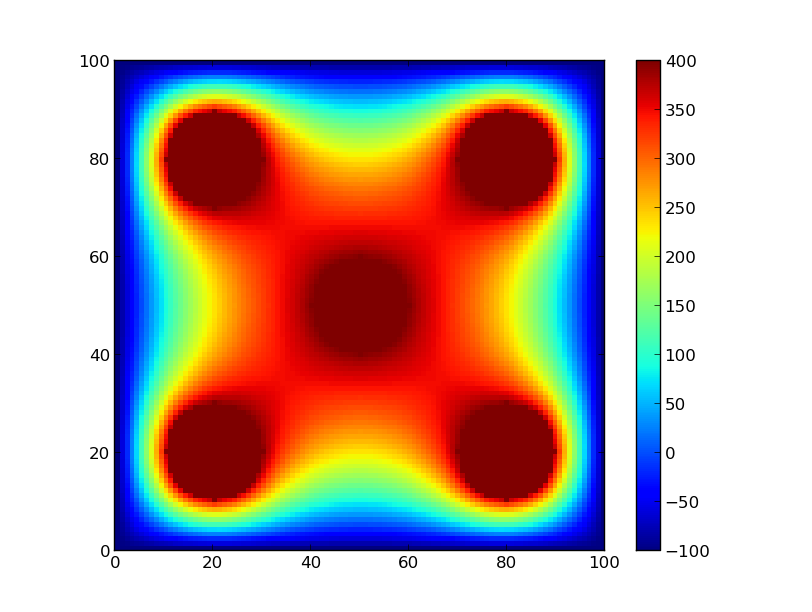
\includegraphics[width=\textwidth]{imagenes/test5_gran1.png}
                \caption{Granularidad 1}
        \end{center}
\endminipage\hfill
\minipage{0.5\textwidth}
\begin{center}
        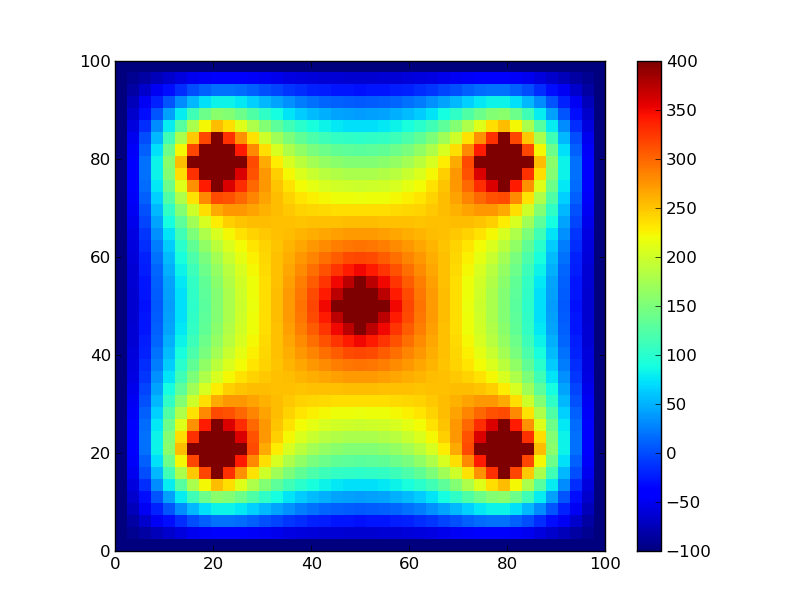
\includegraphics[width=\textwidth]{imagenes/test5.png}
                \caption{Granularidad 2.5}
        \end{center}
\endminipage\hfill 
\end{figure}

\begin{figure}[!htb]
\minipage{0.5\textwidth}
\begin{center}
    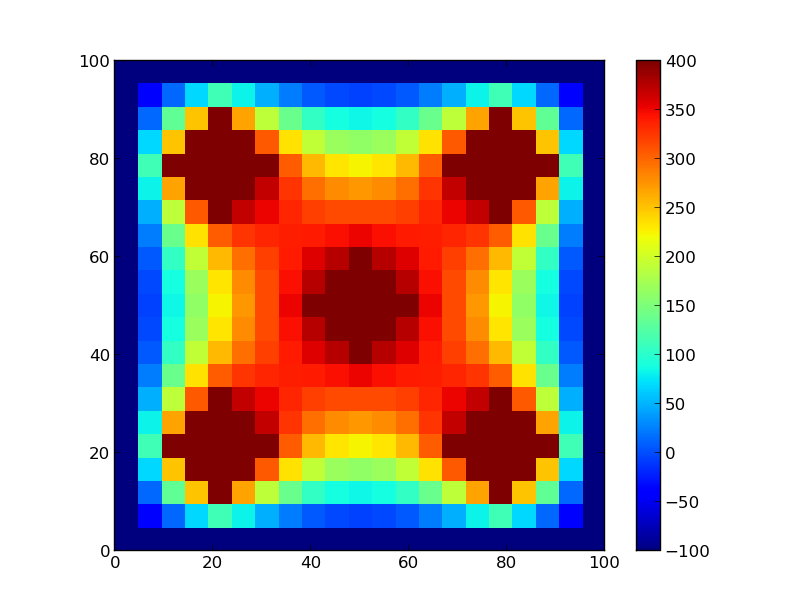
\includegraphics[width=\textwidth]{imagenes/test5_gran5.png}
                \caption{Granularidad 5}
 \end{center}
\endminipage
\minipage{0.5\textwidth}
\begin{center}
   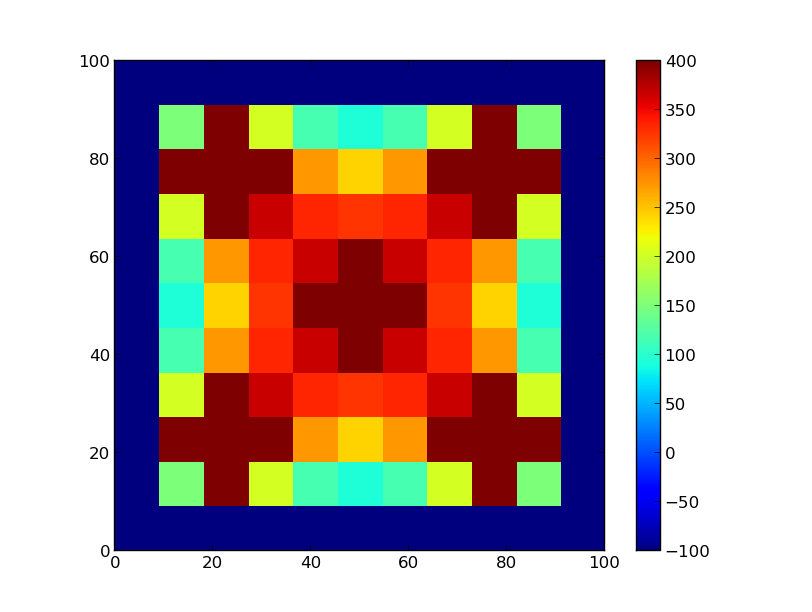
\includegraphics[width=\textwidth]{imagenes/test5_gran10.png}
                \caption{Granularidad 10}
        \end{center}
\endminipage\hfill
\end{figure}

Ahora veamos que obtenemos al aplicarle distintas veces el algoritmo de solución random explicado en el desarrollo (\ref{sec:solucionRandom}).
\newpage

\begin{figure}[htb]
\begin{center}
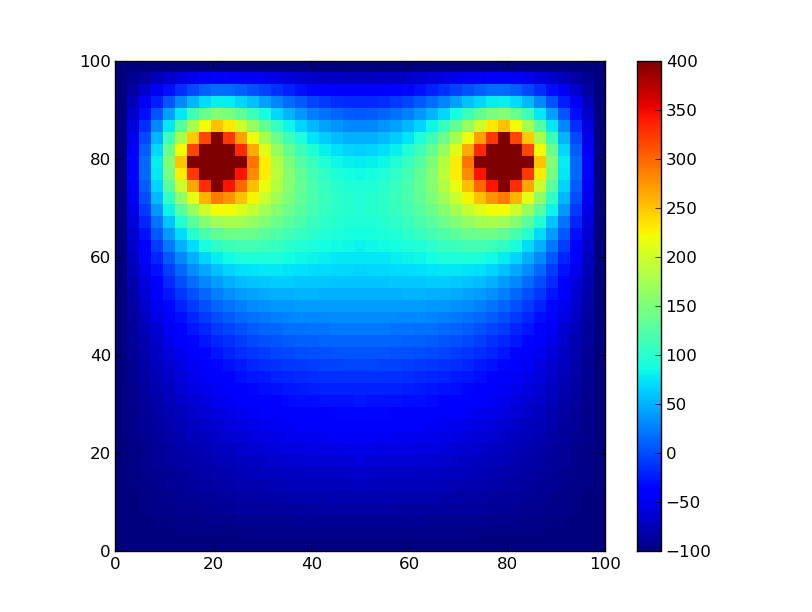
\includegraphics[scale=0.50]{imagenes/random_1.png} 
\caption{Resultado primer corrida} 
\end{center}
\end{figure}


\begin{figure}[htb]
\begin{center}
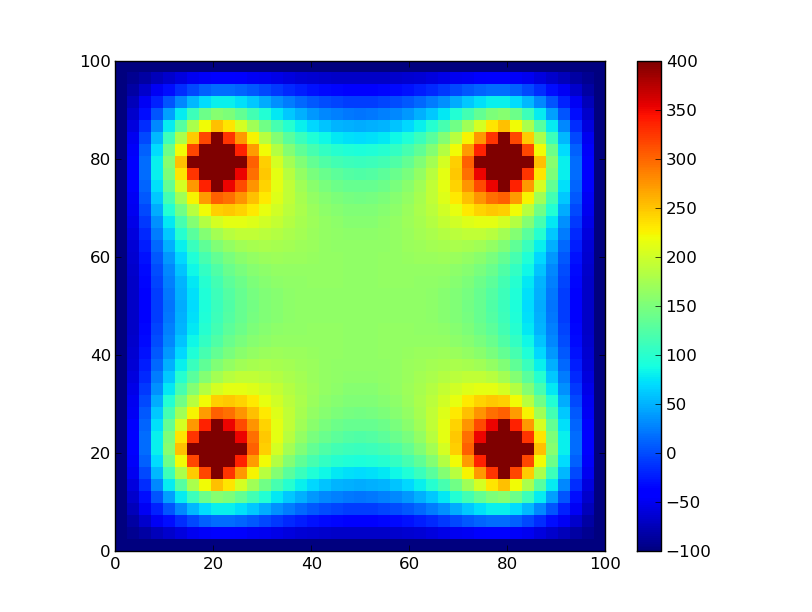
\includegraphics[scale=0.50]{imagenes/random_2.png} 
\caption{Resultado segunda corrida} 
\end{center}
\end{figure}
\newpage

\begin{figure}[htb]
\begin{center}
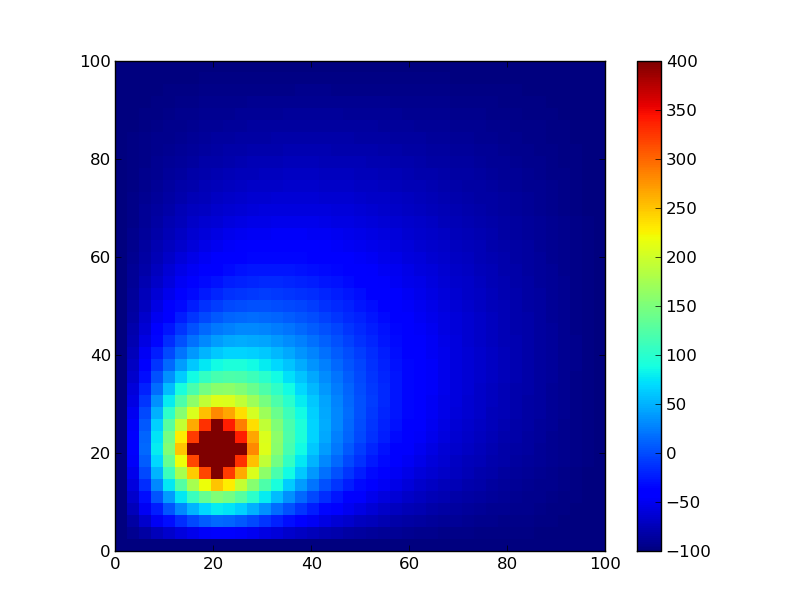
\includegraphics[scale=0.50]{imagenes/random_3.png} 
\caption{Resultado tercer corrida} 
\end{center}
\end{figure}

Como podemos observar la solución óptima (la que menos sanguijuelas elimina), es la segunda. Pero como esta solución es completamente random en la primera corrida mata 2 sanguijuelas antes de elegir la correcta y en la tercera 4. Sólo en la segunda elije en el primer intento la sanguijuela correcta.

\newpage



\subsection{Resultados Greedy}

Veamos ahora para la misma matriz como se comporta nuestro otro algoritmo. 


\begin{figure}[htb]
\begin{center}
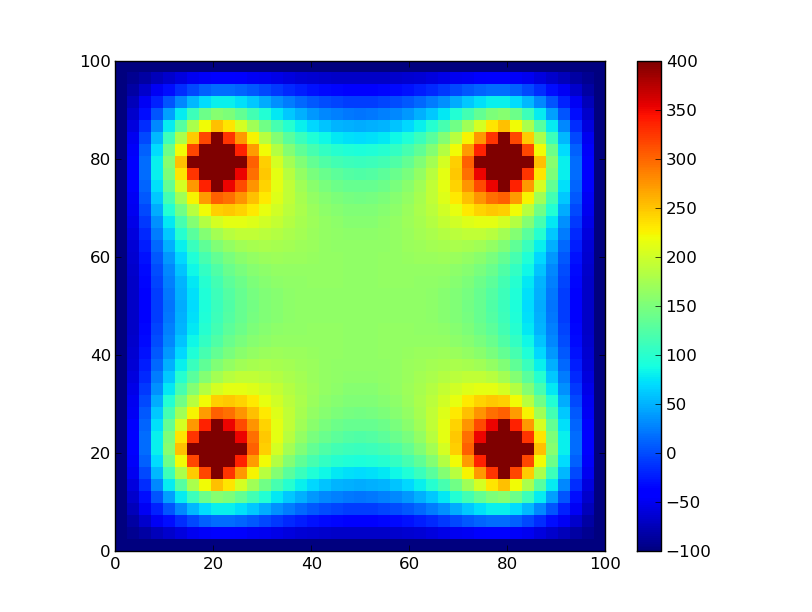
\includegraphics[scale=0.40]{imagenes/random_2.png} 
\caption{Resultado corrida con greedy} 
\end{center}
\end{figure}


En todas las corridas obtuvimos el mismo resultado y demoraron lo mismo. Era de esperarse, ya que efectivamente en este caso, la sanguijuela a eliminar era la del medio.
\newpage
\subsection{Resultados Banda VS Gaussiano}
Veamos ahora que realmente valió la pena la mejora al saber que era matriz banda en cuanto a tiempos en comparación con la eliminación gaussiana.
Anotamos que agregar un análisis de resultados no vale la pena ya que son el mismo

\begin{figure}[htb]
\begin{center}
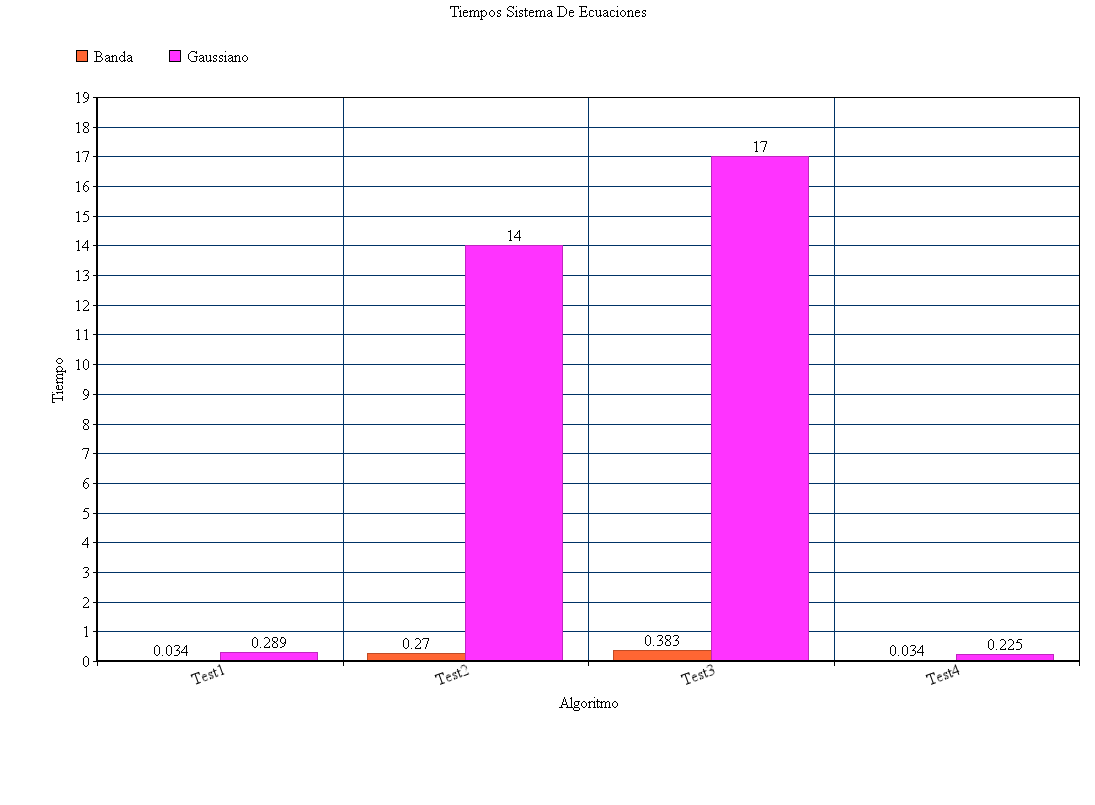
\includegraphics[scale=0.50]{imagenes/tiemposGaussVsBanda.png} 
\caption{Gauss VS Banda} 
\end{center}
\end{figure}
